\documentclass{beamer}

% Theme
\usetheme{Madrid}
\usecolortheme{default}

% Packages
\usepackage{amsmath,amssymb,amsfonts}
\usepackage{gvv}
\usepackage{graphicx}
\usepackage{xcolor}
\usepackage{tikz}
\usepackage{tkz-euclide}
\usepackage{array}
\usepackage{multirow}
\usepackage{longtable}
\usepackage{lscape}
\usepackage{listings}
\lstset{
    basicstyle=\ttfamily\small,
    keywordstyle=\color{blue},
    commentstyle=\color{gray},
    stringstyle=\color{red},
    showstringspaces=false,
    breaklines=true
}
% Redefine \vec to bold letters only (no arrow)
\renewcommand{\vec}[1]{\mathbf{#1}}

\title{4.10.21}
\author{EE25BTECH11019 -- Darji Vivek M.}
\date{}

\begin{document}

\begin{frame}
\titlepage
\end{frame}

\begin{frame}{Question}
\textbf{Question}:\\
Prove that the line through $A(0,-1,-1)$ and $B(4,5,1)$ intersects the line through $C(3,9,4)$ and $D(-4,4,4)$.\\[4pt]
\end{frame}

\begin{frame}{Solution}

\textbf{Matrix Method:}\\
\begin{align}
\vec{A}&=\myvec{0\\-1\\-1},\quad
\vec{B}=\myvec{4\\5\\1},\quad
\vec{C}=\myvec{3\\9\\4},\quad
\vec{D}=\myvec{-4\\4\\4},\\
\vec{d}_1&=\vec{B}-\vec{A}=\myvec{4\\6\\2},\quad
\vec{d}_2=\vec{D}-\vec{C}=\myvec{-7\\-5\\0},\\
\vec{P}(\lambda)&=\vec{A}+\lambda\vec{d}_1,\quad
\vec{Q}(\mu)=\vec{C}+\mu\vec{d}_2,\\
\vec{P}(\lambda)&=\vec{Q}(\mu)\implies 
\lambda\vec{d}_1-\mu\vec{d}_2=\vec{C}-\vec{A},\\
\vec{C}-\vec{A}&=\myvec{3\\10\\5}.
\end{align}
\end{frame}

\begin{frame}{Solution}
\textbf{Formulating as a Matrix Equation:}
\begin{align}
\myvec{\vec{d}_1 & -\vec{d}_2}\myvec{\lambda\\\mu}=\vec{C}-\vec{A}.
\end{align}

Substituting the values,
\begin{align}
\myvec{4 & 7\\6 & 5\\2 & 0}\myvec{\lambda\\\mu}=\myvec{3\\10\\5}.
\end{align}
\end{frame}

\begin{frame}{Solution}
Augmented matrix and row-reduction: 
\begin{equation}
\resizebox{1\textwidth}{!}{$
\augvec{2}{3}{4 & 7 & 3\\ 6 & 5 & 10\\ 2 & 0 & 5}
\xrightarrow{R_1 \leftrightarrow R_3,\ R_3 \rightarrow R_3 - 2R_1}
\augvec{2}{3}{2 & 0 & 5\\ 6 & 5 & 10\\ 4 & 7 & 3}
\xrightarrow{R_1 \rightarrow \tfrac{1}{2}R_1,\ R_2 \rightarrow R_2 - 6R_1,\ R_3 \rightarrow R_3 - 4R_1}
\augvec{2}{3}{1 & 0 & \tfrac{5}{2}\\ 0 & 5 & -5\\ 0 & 7 & -7}
\xrightarrow{R_2 \rightarrow \tfrac{1}{5}R_2,\ R_3 \rightarrow R_3 - \tfrac{7}{5}R_2}
\augvec{2}{3}{1 & 0 & \tfrac{5}{2}\\ 0 & 1 & -1\\ 0 & 0 & 0}
$}

\end{equation}
From the reduced system we read off
\begin{align}
\lambda &= \tfrac{5}{2},\\
\mu     &= -1.
\end{align}
\end{frame}

\begin{frame}{Intersection Point}
Intersection point:
\begin{align}
\vec{P}\!\left(\tfrac{5}{2}\right)
&=\myvec{0\\-1\\-1}+\tfrac{5}{2}\myvec{4\\6\\2}
=\myvec{10\\14\\4},\\
\vec{Q}(-1)
&=\myvec{3\\9\\4}+(-1)\myvec{-7\\-5\\0}
=\myvec{10\\14\\4}.
\end{align}

\text{Therefore, the lines intersect at }
\boxed{\myvec{10\\14\\4}}.
\end{frame}

\begin{frame}[fragile]{C Code}
\begin{lstlisting}
#include <stdio.h>
#include <math.h>

// Function: check intersection of line AB and line CD
// Returns 1 if they intersect, else 0
int line_intersection(double A[3], double B[3], double C[3], double D[3], double P[3]) {
    double d1[3], d2[3], rhs[3];
    double a11, a12, a21, a22, b1, b2, det;
    double lambda, mu;

    // direction vectors
    d1[0] = B[0] - A[0];
    d1[1] = B[1] - A[1];
    d1[2] = B[2] - A[2];

    d2[0] = D[0] - C[0];
    d2[1] = D[1] - C[1];
    d2[2] = D[2] - C[2];
\end{lstlisting}
\end{frame}

\begin{frame}[fragile]{C Code}
\begin{lstlisting}
    // rhs = C - A
    rhs[0] = C[0] - A[0];
    rhs[1] = C[1] - A[1];
    rhs[2] = C[2] - A[2];
  // Build 2x2 system using dot products (Gram matrix)
    a11 = d1[0]*d1[0] + d1[1]*d1[1] + d1[2]*d1[2];
    a12 = d1[0]*d2[0] + d1[1]*d2[1] + d1[2]*d2[2];
    a21 = a12;
    a22 = d2[0]*d2[0] + d2[1]*d2[1] + d2[2]*d2[2];

    b1 = d1[0]*rhs[0] + d1[1]*rhs[1] + d1[2]*rhs[2];
    b2 = d2[0]*rhs[0] + d2[1]*rhs[1] + d2[2]*rhs[2];

    det = a11*a22 - a12*a21;
    if(fabs(det) < 1e-6) return 0; // parallel

    lambda = ( b1*a22 - b2*a12 ) / det;
    mu     = ( a11*b2 - a21*b1 ) / det;

\end{lstlisting}
\end{frame}


\begin{frame}[fragile]{C Code}
\begin{lstlisting}
  // Intersection point from line AB
    P[0] = A[0] + lambda*d1[0];
    P[1] = A[1] + lambda*d1[1];
    P[2] = A[2] + lambda*d1[2];

    // Point from line CD
    double Q[3];
    Q[0] = C[0] + mu*d2[0];
    Q[1] = C[1] + mu*d2[1];
    Q[2] = C[2] + mu*d2[2];

    // Check if P == Q
    if(fabs(P[0]-Q[0]) < 1e-6 && fabs(P[1]-Q[1]) < 1e-6 && fabs(P[2]-Q[2]) < 1e-6)
        return 1;
    return 0;
}

\end{lstlisting}
\end{frame}
%-------------------------------
\begin{frame}[fragile]{Python (Call)}
\begin{lstlisting}[language=Python]
import ctypes
import numpy as np
import matplotlib.pyplot as plt

# Load shared C library
lib = ctypes.CDLL("./8.so")

# Define argument and return types
lib.line_intersection.argtypes = [ctypes.POINTER(ctypes.c_double), ctypes.POINTER(ctypes.c_double),
                                  ctypes.POINTER(ctypes.c_double), ctypes.POINTER(ctypes.c_double),
                                  ctypes.POINTER(ctypes.c_double)]
lib.line_intersection.restype = ctypes.c_int
\end{lstlisting}
\end{frame}

\begin{frame}[fragile]{Python (Call)}
\begin{lstlisting}[language=Python]
# Points
A = np.array([0, -1, -1], dtype=np.double)
B = np.array([4,  5,  1], dtype=np.double)
C = np.array([3,  9,  4], dtype=np.double)
D = np.array([-4, 4,  4], dtype=np.double)
P = np.zeros(3, dtype=np.double)

# Call C function
res = lib.line_intersection(A.ctypes.data_as(ctypes.POINTER(ctypes.c_double)),
                            B.ctypes.data_as(ctypes.POINTER(ctypes.c_double)),
                            C.ctypes.data_as(ctypes.POINTER(ctypes.c_double)),
                            D.ctypes.data_as(ctypes.POINTER(ctypes.c_double)),
                           
\end{lstlisting}
\end{frame}

\begin{frame}[fragile]{Python (Call)}
\begin{lstlisting}[language=Python]
                             P.ctypes.data_as(ctypes.POINTER(ctypes.c_double)))

print("Intersect:", bool(res))
if res:
    print("Intersection Point:", P)

# ---- Plot ----
fig = plt.figure()
ax = fig.add_subplot(111, projection="3d")
# Line AB
ax.plot([A[0], B[0]], [A[1], B[1]], [A[2], B[2]], 'r', label="Line AB")
\end{lstlisting}
\end{frame}

\begin{frame}[fragile]{Python (Plot)}
\begin{lstlisting}[language=Python]
ax.text(*A, "A")
ax.text(*B, "B")

# Line CD
ax.plot([C[0], D[0]], [C[1], D[1]], [C[2], D[2]], 'b', label="Line CD")
ax.text(*C, "C")
ax.text(*D, "D")

# Intersection point
if res:
    ax.scatter(P[0], P[1], P[2], color='g', s=50, label="Intersection P")
    ax.text(*P, "P")

ax.legend()
plt.show()


\end{lstlisting}
\end{frame}

\begin{frame}{Python Output and Plot}
\begin{figure}[h!]
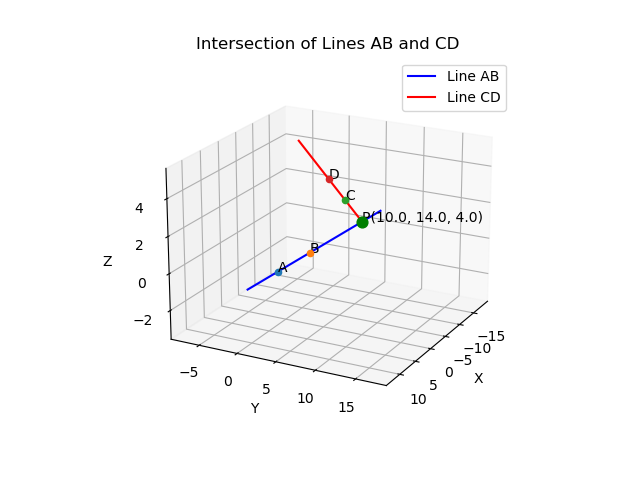
\includegraphics[width=0.75\columnwidth]{figs/8.png}
\caption{Given 2 lines are Intersecting}
\end{figure}
\end{frame}

\end{document}
